\section{Perceptron} \label{sc:per}

\subsection{Aufbau und Notation}

Im Jahr 1958 entwickelte der US-amerikanische Psychologe und Informatiker Frank Rosenblatt das sogenannte \emph{Perceptron}. Dieses stellt das älteste neuronale Netz dar, welches teilweise auch heutzutage noch genutzt wird. Inspiriert wurde Rosenblatt vom Auge einer Fliege, wobei die Entscheidung der nächsten Flugrichtung in Teilen bereits im Auge stattfindet. Das Perceptron stellt in diesem Zusammenhang eine direkte Abbildung dieser Beobachtung dar.

Das Modell ist eine Weiterentwicklung von der McCulloch-Pitts-Zelle (siehe \autoref{sc:mpn}). Allerdings ist das Perceptron in der Lage die unterschiedlichen Eingabewerte zu priorisieren. Dies geschieht mittels reeller Gewichte, welche jeweils mit den Inputwerten verrechnet werden: $\sum_j w_j x_j$. Gleich bleibt jedoch die binäre Klassifizierung, wie schon bei der McMulloch-Pitts-Zelle.

\begin{figure}[!htb]
	\centering
	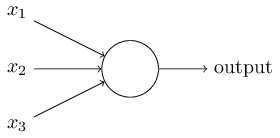
\includegraphics[width=.5\linewidth]{./img/erstesPerceptron}
	\mycaption{Perceptron - drei Eingabewerte}{dlnielsen}
	\label{fig:erstesPerceptron}
\end{figure}

Die Abbildung \ref{fig:erstesPerceptron} beschreibt ein einfaches Perceptron mit drei Eingabewerten. Genau wie die MP-Zelle verwendet dieses Modell einen Schwellwert $\theta$ um den letztendlichen Ausgabewert zu bestimmen, jedoch möchte ich hier noch einmal etwas genauer auf die Notation des Ganzen eingehen, da diese auch in späteren Abschnitten benötigt wird.

Die Funktion, welche berechnet, ob ein Schwellwert überschritten wird oder nicht, wird \emph{Aktivierungsfunktion} genannt (hier mit \emph{g} bezeichnet).

\begin{equation} \label{eq:aktFkt}
g(\mathbf{z}) =\begin{cases}
	0 & \mbox{if } \mathbf{z} \leq \theta \\
    1 & \mbox{if } \mathbf{z} > \theta
  \end{cases}
\end{equation}

wobei gilt

\begin{equation} \label{eq:vektorprod}
\mathbf{w} = \begin{bmatrix}
    w_{1}  \\
    \vdots \\
    w_{m}
\end{bmatrix}
\quad  \mathbf{x} = \begin{bmatrix}
    x_{1}  \\
    \vdots \\
    x_{m}
\end{bmatrix}
\end{equation}

\begin{equation}
\mathbf{z} =  w_1x_{1} + \dots + w_mx_{m} = \sum_{j=1}^{m} x_{j}w_{j} \\ = \mathbf{w}^T\mathbf{x}
\end{equation}

Sämtliche Gewichte und Eingabewerte können als Vektoren betrachtet werden. Die Summe der Produkte kann dadurch wiederum schlicht als \emph{Vektorpunktprodukt} verstanden werden (siehe \autoref{eq:vektorprod}).

Um die generelle Notation des gesamten Modells zu vereinfachen bietet es sich außerdem an den Schwellwert $\theta$ auf die linke Seite der Gleichung (siehe Gleichung \ref{eq:aktFkt}) zu ziehen. Damit gelten folgende Rahmenbedingungen:

\begin{equation} \label{eq:aktFkt2}
g(\mathbf{z}) =\begin{cases}
	0 & \mbox{if } \mathbf{z} \leq 0 \\
    1 & \mbox{if } \mathbf{z} > 0
  \end{cases}
\end{equation}

wobei gilt

\begin{equation} \label{eq:vektorprod}
z =  \mathbf{w_0x_{0}} + w_1x_{1} + \dots + w_mx_{m} = \sum_{j=0}^{m} x_{j}w_{j} \\ = w^Tx
\end{equation}

\label{w0Erklaerung}
Wichtig hierbei, es wird ein zusätzliches Gewicht welches den negativen Schwellwert hält, sowie einen zusätzlichen Inputwert mit dem Wert 1, eingeführt ($w_0 = -\theta  \text{ und } x_0=1$). Bei der Berechnung (siehe \autoref{eq:aktFkt2}) fließt dieser Faktor nun als negativer Summand mit ein wodurch man nur noch prüft ob die Gesamtsumme kleiner Null ist oder nicht. Von dieser Notation wird insbesondere bei der \emph{Lernregel} (siehe Abschnitt \ref{ss:lernregel}) Gebrauch gemacht. Mittels dieser Vereinfachung lässt sich ein Modell auch folgendermaßen darstellen:

\begin{figure}[!htb]
	\centering
	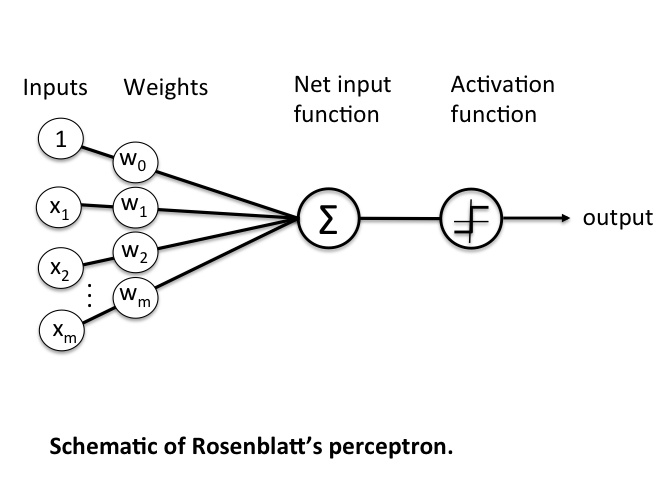
\includegraphics[width=.6\linewidth]{img/perceptron_schematisch}
	\mycaption{Perceptron - Modelansicht}{mpNeuron}
	\label{fig:perc_modelansicht}
\end{figure}

\FloatBarrier

Letztendlich sei jedoch erwähnt, dass es in der Literatur auch öfters eine Darstellung mittels eines Schwellwerts (engl. \emph{Bias}) gibt, siehe Gleichung \autoref{eq:aktFkt3} \cite{dlnielsen}

\begin{equation} \label{eq:aktFkt3}
\mbox{output} =\begin{cases}
	0 & \mbox{if } w\cdot x + b \leq 0 \\
    1 & \mbox{if } w\cdot x + b > 0
  \end{cases}
\end{equation}



\subsection{Lernregel} \label{ss:lernregel}

\paragraph{Erklärung}

Das bisher vorgestellte Modell beinhaltet bis jetzt wenig Eigenschaften für einen \emph{lernenden} Algorithmus, dies ändert sich jedoch mit der Idee von Rosenblatt das Modell selbst die Angleichung der Gewichte übernehmen zu lassen. Hierzu wird auf eine Menge von Trainingsdatensätzen zurückgegriffen.
Diese Datensätze bestehen aus Eingabewerten für das System und der korrespondierenden Ausgabe. Die Lernregel selbst sieht zusammengefasst folgendermaßen aus.

\vspace{4mm}
\begin{minipage}{\textwidth}
\begin{itemize}
\item Initialisiere die Gewichte mit einem sehr kleinen Wert oder dem Wert 0.
\item Für jeden Datensatz der Menge:
\begin{itemize}
	\item Berechne den Ausgabewert des Systems
	\item Gleiche die Gewichte an
\end{itemize}
\end{itemize}
\end{minipage}

\vspace{5 mm}

\label{sp:lernrate}
Der genannte Ausgabewert wird über die Aktivierungsfunktion des Modells bestimmt. Die einzelnen Komponenten des \emph{Gewichtevektors} werden getrennt betrachtet und angeglichen. Ein Aktualisieren eines einzelnen Gewichts innerhalb des Gewichtsvektors wird formal mit $w_j := w_j + \Delta w_j$ beschrieben (das Delta kennzeichnet, dass es sich um eine \emph{Veränderung} handelt). Da die beschriebene Lernregel inkrementell arbeitet, muss man eine sogenannte \emph{Lernrate} bestimmen. Dieser Wert bestimmt letztendlich, wie stark ein Gewicht bei einer Iteration verändert wird. Formal wird diese Rate mit dem Zeichen $\eta$ dargestellt. Die allgemeine Darstellung zum Angleichen der Gewichte sieht folgendermaßen aus:

\begin{equation} \label{eq:lernRegel}
\Delta w_j = \eta \; (\text{target}^{(i)} - \text{output}^{(i)})\;x^{(i)}_{j}
\end{equation}

Zuerst wird ein Datensatz gewählt durch dessen Ausgabewerte alle Gewichte angeglichen werden sollen. Generell gilt, dass das \emph{i} in den Klammern nicht als Exponent, sondern als Index für den betrachteten Trainingsdatensatz steht. Dann wird die Differenz des optimalen Ausgabewerts und des erreichten Werts berechnet. Diese Differenz wird anschließend mit der Lernrate und dem korrespondierenden Eingabewert des betrachteten Gewichts multipliziert. Dies wird vielleicht etwas klarer, wenn man noch einmal einen Blick in das Diagramm \ref{fig:perc_modelansicht} auf Seite \pageref{fig:perc_modelansicht} wirft. Der Eingabewert $x^{(i)}_{j}$ steht also für die Komponente mit dem Index \emph{j} in dem Eingabevektor des Trainingsdatensatzes an der Stelle \emph{i} innerhalb der Menge von Trainingsdaten.


\paragraph{Anwendung}

Für einen zweidimensionalen Trainingsdatensatz\footnote{Ein zweidimensionaler Datenpunkt besitzt einen zweidimensionalen Eingabevektor (also genau zwei Eingabewerte).} würde die Lernregel folgendermaßen aussehen. Hervorzuheben sei jedoch, dass alle Gewichte gleichzeitig angeglichen werden.

\begin{equation} \label{eq:lernRegAnw}
\begin{aligned}
& \Delta w_0 = \eta(\text{target}^{(i)} - \text{output}^{(i)}) \\
& \Delta w_1 = \eta(\text{target}^{(i)} - \text{output}^{(i)})\;x^{(i)}_{1} \\
& \Delta w_2 = \eta(\text{target}^{(i)} - \text{output}^{(i)})\;x^{(i)}_{2}
\end{aligned}
\end{equation}

In dieser Darstellung wurde die bereits in \ref{w0Erklaerung} besprochene Notation verwendet bei der ein zusätzliches Gewicht mit dem Schwellwert eingeführt wurde. Da der eigentliche Eingabewert hierbei lediglich den Faktor \emph{1} besitzt, fällt er hierbei einfach weg. Wir haben also neben diesem einbezogenen \emph{Bias} lediglich die zwei weitere Gewichte, die angeglichen werden.

Für den Fall, dass das Modell einen Datensatz richtig klassifiziert gibt es genau zwei Möglichkeiten:

\begin{equation}
\begin{aligned}
& \Delta w_j = \eta \big( (-1^{(i)}) - (-1^{(i)}) \big)\;x^{(i)}_{j} = 0 \\
& \Delta w_j = \eta(1^{(i)} - 1^{(i)})\;x^{(i)}_{j} = 0 \\
\end{aligned}
\end{equation}

Durch den Differenzfaktor von Null verändert sich das betrachtete Gewicht erwartungsgemäß nicht. Bei dem entsprechenden Gegenteil ist dies nicht der Fall, hier könnte es zum Beispiel so aussehen:

\begin{equation}
\begin{aligned}
& \Delta w_j = \eta \big( 1^{(i)} - (-1^{(i)}) \big) \;x^{(i)}_{j} = \eta(2)\;x^{(i)}_{j} \\
& \Delta w_j = \eta \big( (-1^{(i)}) - 1^{(i)} \big) \;x^{(i)}_{j} = \eta(-2)\;x^{(i)}_{j} \\
\end{aligned}
\end{equation}


% & \Delta w_j = \eta \big( 1^{(i)} - (-1^{(i)}) \big) \;x^{(i)}_{j} = \eta(2)\;x^{(i)}_{j} \\
% & \Delta w_j = \eta \big( (-1^{(i)}) - 1^{(i)} )\big \;x^{(i)}_{j} = \eta(-2)\;x^{(i)}_{j} \\

Eine Implementierung des beschriebenen Konzepts in der Programmiersprache Python ist auf Github \cite{pcImplementierung} zu finden. Ich werde hier jedoch nicht weiter auf die Details der Implementierung eingehen.

Wie schon die McCulloch-Pitts Zelle (siehe Abbildung \ref{fig:aufbau} Seite \pageref{fig:aufbau}) ist das Perceptron nur in der Lage mittels einer linearen Klassifizierungs-Funktion die zwei unterschiedlichen Gruppen auseinander zu halten (siehe Abbildung \ref{fig:probKlassi}).

\FloatBarrier

\begin{figure}[htb!]
  \centering
  \subfloat[][]{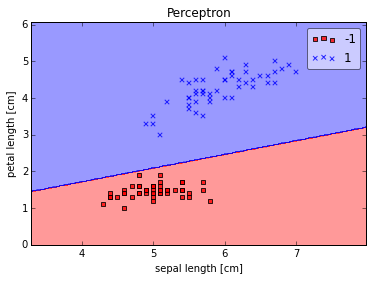
\includegraphics[width=.39\linewidth]{img/perceptron_klassifizierung1}}
  \qquad
  \subfloat[][]{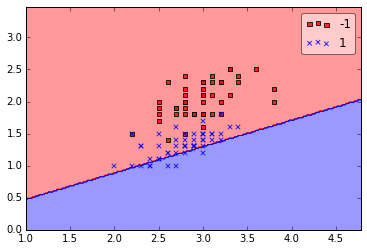
\includegraphics[width=.405\linewidth]{img/perceptron_klassifizierung2}}%
  % todo zweite Quelle mit in Macro einbinden
  \mycaption{Perceptor - Problematische Klassifizierung}{mpNeuron}
  \label{fig:probKlassi}
\end{figure}
